\documentclass{article}
\usepackage[utf8]{inputenc}
\usepackage[margin=0.45in]{geometry}
\usepackage{amsmath}
\usepackage{ dsfont }
\usepackage{wrapfig}
\usepackage{graphicx}
\graphicspath{ {images/} }
\usepackage{subfig}

\title{ORIE 4741: Project Midterm Report}
\author{Ryan Butler, Dae Won Kim, Peiyun Zhang}
\date{\today}
\setlength{\parindent}{0pt}

\begin{document}
\maketitle

\section{Introduction}
Yelp is a review-sharing platform, in which users actively archive numeric evaluations of businesses in the form of a star rating and provide context by text. The reviews are then further evaluated by other users, who can choose to tag each review post as "funny","cool", or "useful." The accumulation of such votes can illustrate the "character" of each review, and analysis on the mapping between the contents of the review and these votes can reveal what determines one's reaction to a block of text and its context. Broadly, such analysis would be similar to sentiment analysis, where positivity of a block of text can be gauged by a numeric feature. However, "funny", "cool", and "useful" are much more complex constructs and are also not mutually exclusive. Our challenge, therefore, will rest on how we define our target predicted variable. It will also rest on how we determine the relative funniness, coolness, and usefulness of a review, and on how we determine an effective numeric transformation of the text data. Our aim is to analyze the effectiveness of ML models - in conjunction with text-to-numeric transformation techniques - in predicting funny, cool, or usefulness, and the effects of both text and non-text features of a review on such predictions. 

\section{Data Preprocessing}
\subsection{Data Acquisition}
Data was obtained from the Yelp Dataset Challenge[https://www.yelp.com/dataset/challenge], which offers several large files that respectively contain information on 4 million reviews, 1 million users who wrote these reviews, and 150,000 businesses. All of our operations for this midterm report were done exclusively on the review file. Note that we intend to incorporate information on users and businesses in our analysis, but our preliminary analysis was primarily focused on text data. The dataset itself contains ids that connect it to the author and business, associated star rating, date of authorship, and votes made by other users. Shown below is the schema of the review dataset: 

\begin{table}[h]
\centering
\begin{tabular}{l l l}
\hline
\textbf{Column Name} & \textbf{Type} & \textbf{Description}\\
\hline
review\_id & string & unique review id \\
user\_id & string & user id of writer of review\\
business\_id & string & unique business id \\
stars & integer & average star rating for a review\\
text & string & review text (typically 200+ words)\\
useful & integer & number of useful votes received\\
funny & integer & number of funny votes received\\
cool & integer & number of cool votes received\\
\hline
\end{tabular}
\caption{Review Dataset Schema}
\end{table}

\subsection{Tools Used}
To process very large text files - gigabytes of it - Apache Spark, the state-of-the-art parallel processing platform was used. It comes with modules on text processing, principal component analysis, and allows scalability of algorithms. We also had access to a Linux cluster with 70 cpu cores, which further improved our computing performance.

For numeric encoding of text information, we used word2vec, a popular word embedding framework that transforms a dictionary matrix - a matrix whose entries correspond to a frequency of a certain word(column) in a certain block of text(row) - using a high-dimensional vector space created by a two-layer neural network. Each word is translated to a numeric vector, and similar words are much close in orientation, and the whole text is an aggregation of these vectors. At a high-level, the word2vec produces from a block of text its "orientation" based on a shared vocabulary. The resulting numeric matrix - made by row-wise concatenation of word2vec transformations - will then be used as input for our ML algorithms.

\subsection{Feature Engineering}
The advantages of this specific dataset is that there are no missing values or invalid values, which comes from the fact that there are very few columns, and many are in fact pre-cleaned by Yelp. Therefore the majority of the preprocessing was done with the text encoding, as well as filtering of data based on two principles: (1) The sum of the votes received for all three categories(cool, useful, funny) is more than 10, (2) The vote received from one categories is at least 50\% of the total vote. These rules allow us to focus on reviews that are predominantly in one category as opposed to the other two categories. We also want enough votes to make sure it's reasonable to use the majority criteria. To do this, we created a new column called “total\_vote" to filter reviews with less than 10 votes. \\

\begin{wrapfigure}{r}{0.4\textwidth}
  %\begin{center}
 	\centerline{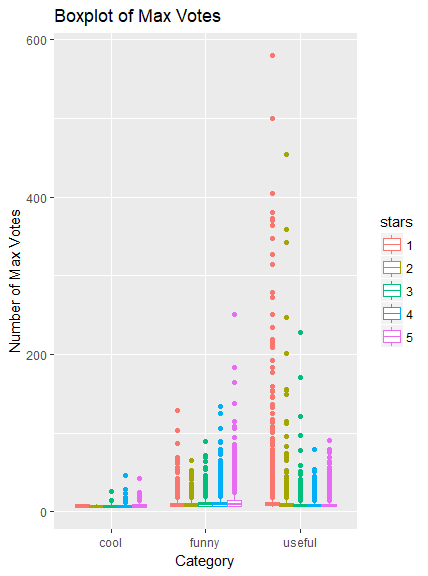
\includegraphics[width=7cm,height=8.9cm,keepaspectratio]{vote_category_boxplot.png}}
  %\end{center}
  \caption{Boxplot of Max Votes}
  %\setlength{\belowcaptionskip}{-10pt}
\end{wrapfigure}
%\setlength{\belowcaptionskip}{-10pt}

For the text encoding, the following steps were made: (1) Convert text to a list of words, (2) Remove stop words ( the, and, a for example), (3) lemmatize words (fast, faster, fastest all become fast, for example) and (4) Create a dictionary matrix based on frequency counts of words. (5) Use Word2Vec module to transform dictionary matrix


\section{Preliminary Analysis}
\subsection{Basic Visualization}
The two filtering principles reduces the 4 million reviews to about 45,000 reviews, which is less than 2\% of the data we started with. Overall, usefulness is the most dominant of these categories, with at least 70\%. We wanted to see if there are obvious factors other than the text that affects voting intensities in the three categories. Figure 1 is the box plot of number of maximum vote for each review grouped by is associated category. From this plot, it is quite obvious that within "useful", negative reviews tend to have higher votes; whereas positive reviews tend to have higher votes within "funny" category. Yet "cool" does not appear to be a popular button at all. Also in general, "useful" receives far more votes than "funny" and "cool" combined. This suggests that the star rating of a review may be a significant factor in determining the perception of usefulness, coolness, or funniness. 

\subsection{Dimension Analysis of Word2Vec}

Word2Vec transformation was used to transform the text data to a 100-dimension vector, which was then fed into principal component analysis(PCA). PCA determines the first component by finding the axis of largest variance, and iteratively determines the next principal component by determining the next axis of largest variance that is orthogonal to all previous principal components. Figure 2 shows the explained variance quickly decays to below 0.1 by the third component. This suggests, among other things, high degree of sparsity in the word2vec transformations as well as the low-rank structure of the word2vec transformation. This means overall the data is only highly variant on certain directions, and overall very clumped together. This indicates strong correlation between the words, which is expected, since set of words used from person to person is most likely very highly correlated. \\\\
Figure 3 is a low-dimensional representation of the word2vec vectors, using three principal components as the axes. The colors represent associated category - with over 50\% of the votes. There is low degree of separability between the three colors. It may be noted, however, that some amount of green does seem to congregate on the right upper side more, and brown color congregates more on the lower left, and yellow overall populating the center (yellow dominates as it represents usefulness, which is 70\% of the data). This peculiarity in the distribution gives some indication as to separability in a higher dimension space. \\\\
\begin{figure}
    \centering
    \begin{minipage}{0.5\textwidth}
        \centering
        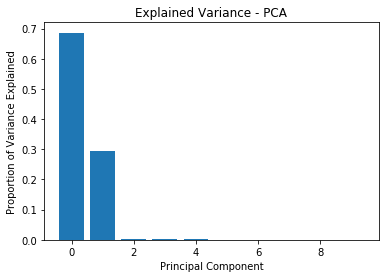
\includegraphics[width=0.9\textwidth]{pca_var.png} 
        \caption{PCA Explained Variance}
    \end{minipage}\hfill
    \begin{minipage}{0.5\textwidth}
        \centering
        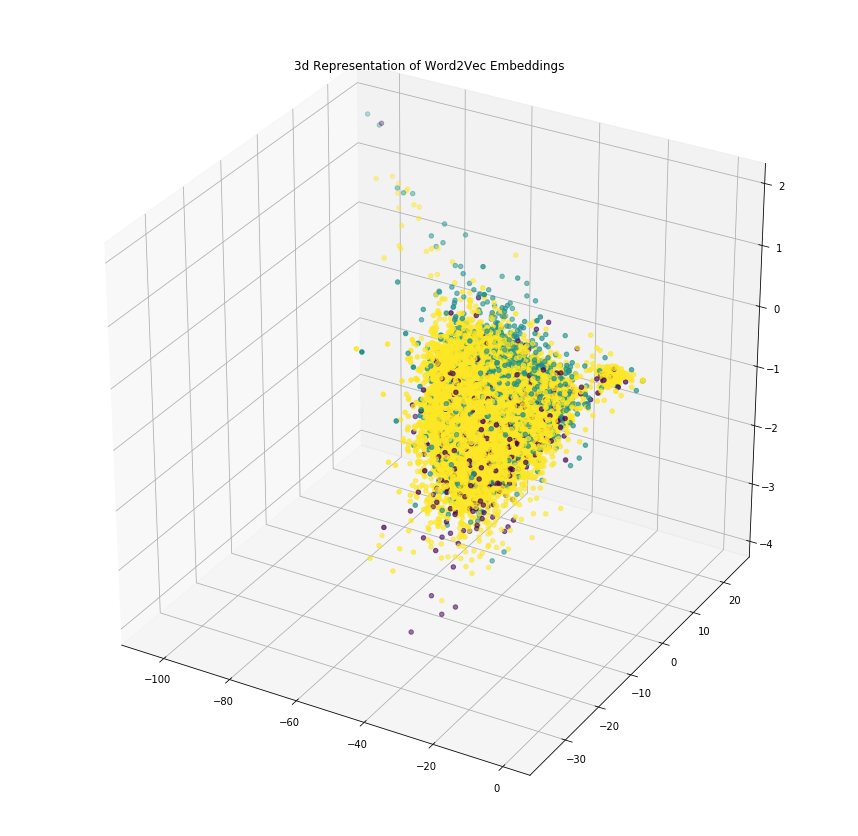
\includegraphics[width=0.9\textwidth]{word2vec_3d.png} 
        \caption{word2vec 3D Representation}
    \end{minipage}
\end{figure}

\section{Evaluation Method}
\subsection{Model Evaluation}
Model evaluation will be done in the following ways, depending on the overall effectiveness of models. We can treat this as a classification problem, where the three classes are "cool","funny", and "useful." Thus we can use things such as precision, recall, F1 score, and area under curve(AUC) as metrics. These values will be obtained using 10-fold cross validation on the data to ensure they are good estimates as to the effectiveness of the data. We can also use the percentage of votes as a target variable for a regression variable. In this case, we will use root mean squared error (RMSE) and absolute deviance as error metrics for evaluation. In this case, we will attempt to minimize the target score.
\subsection{Bias and Variance control}
Word embeddings can be prone to overfitting due to the high correlation between the dimensions. Additionally, as is evident from the PCA analysis and figure 1, it seems there are many other factors at play besides the text, which means more metafeatures on text, and other business, user-related features may need to be introduced. This increased dimension further increases the risk of higher variance of our model and overfitting. This means that when using ML models onto this space should be used with regularization. L1 (Lasso) regularization may be able to perform both feature selection and regularization at the same time, and may be suitable to use. 

\section{Future Work}
\subsection{Data}
As for now, we only had the chance to look at the "review" dataset provided by Yelp. In our next step, we will include (1) "business" dataset, which Contains business data including location data, restaurant attributes, and food categories, and (2) "user" dataset, which contains all the meta-data associated with the users. By doing this, we will have more predictors available for future model construction and analysis.

\subsection{Analysis}
PCA with kernels could be used to further test the separability of the three categories in the feature space. The effectiveness of these transformation techniques will be gauged together with their compatibility to ML models such as logistic regression, decision trees, and SVMs.
We also intend to explore Long Short Term Memory neural nets to do this classification, since they are well-known for their effectiveness in natural language processing, as well as the Neural Turning Machine if time permits. Because recurrent neural network architectures are well suited for sequence data such as text, they should perform well when classifying the data. Several models can be implemented and analyzed, and the best one will be selected for use via cross-validation.



%pca_var.png
%word2vec_3d.png
%vote_category_boxplot.png






\end{document}

